\documentclass[12pt,oneside,a4paper]{article}

\usepackage[backend=biber,style=numeric]{biblatex}
\usepackage{xcolor}
\usepackage{todonotes}
\usepackage{amsmath}
\usepackage{multicol}
\usepackage{caption}
\usepackage{hyperref}
\usepackage{graphicx}
\usepackage{listings}
\lstset{
	frame=top,frame=bottom,
	language=C,
	basicstyle=\small\normalfont,
	xleftmargin=\parindent,
	keywordstyle=\color{green!40!black},
	%  commentstyle=\itshape\color{purple!40!black},
	%  identifierstyle=\color{blue},
	%  stringstyle=\color{orange},
	morekeywords={in, globaldata, procedure, input, output, behavior, end, XOR, NOT, AND}, % keyword to highlight
	%  captionpos=t,
	tabsize=2,
	numbers=left,
	stepnumber=1,                   % the step between two line-numbers.        
	numbersep=5pt,
	framexleftmargin=10pt,
	title=\lstname,
	captionpos=t,
	showspaces=false,
}
\DeclareCaptionFormat{listing}{\rule{\dimexpr\textwidth\relax}{0.4pt}\par\vskip1pt#1#2#3}
\captionsetup[lstlisting]{format=listing,singlelinecheck=false, margin=0pt,labelsep=space,labelfont=bf}

\usepackage{booktabs}
\usepackage[noabbrev,capitalise]{cleveref}
\crefname{listing}{algorithm}{algorithms}
\Crefname{listing}{Algorithm}{Algorithms}
\renewcommand\lstlistingname{Algorithm}
\def\lstlistingcrefname{Algorithm}
\usepackage{url}

\addbibresource{biblio.bib}

\title{\textbf{Spartan and Learning NL2 \\ Accept what you cannot control, work with what you can}}

\author{Camilla Casiraghi}

\date{2023}

\begin{document}


\begin{titlepage}
	\centering
	\clearpage
	\maketitle
	\thispagestyle{empty}
	\vspace*{1cm}
	\vfill
	\centering
	
\includegraphics{logo_polimi.png}
\includegraphics{logo_NECST.png}
\end{titlepage}


\begin{abstract}
This paper goes into the concept of control and the interplay between Spartan races and learning. It explores the aspects that individuals can control and those that are beyond their control. Spartan races, sporting events that involve obstacle course races of varying distances and difficulties, serve as a backdrop for understanding personal agency. The races emphasize the combination of individual challenges and teamwork. This article examines the similarities between the different types of Spartan races and various levels of learning, highlighting how both require commitment, personal challenges, and strategic preparation. It delves into the concept of deliberate practice and performance, emphasizing the importance of setting appropriate objectives and having the right mindset in both Spartan races and academic pursuits, despite what we can't control. By focusing on what can be controlled and maintaining a proactive mindset, individuals can navigate the unpredictable aspects effectively. Ultimately, by choosing to embrace unfamiliar experiences and exercising agency over what is within their control, individuals can enhance their potential and cultivate new learning opportunities.
\end{abstract}

\section{Introduction} \label{sec:intro}
Physical activity holds a significant place in the NecstCAMP pyramid, just below the realm of learning. Activities such as Spartan races can be compared to academic courses at the Politecnico. But what connects the world of Spartan races to the academic environment? In this paper, we will explore the parallelism between Spartan races and learning, highlighting their common elements and how they contribute to personal growth and achievement.
\begin{figure}[h]
    \centering
    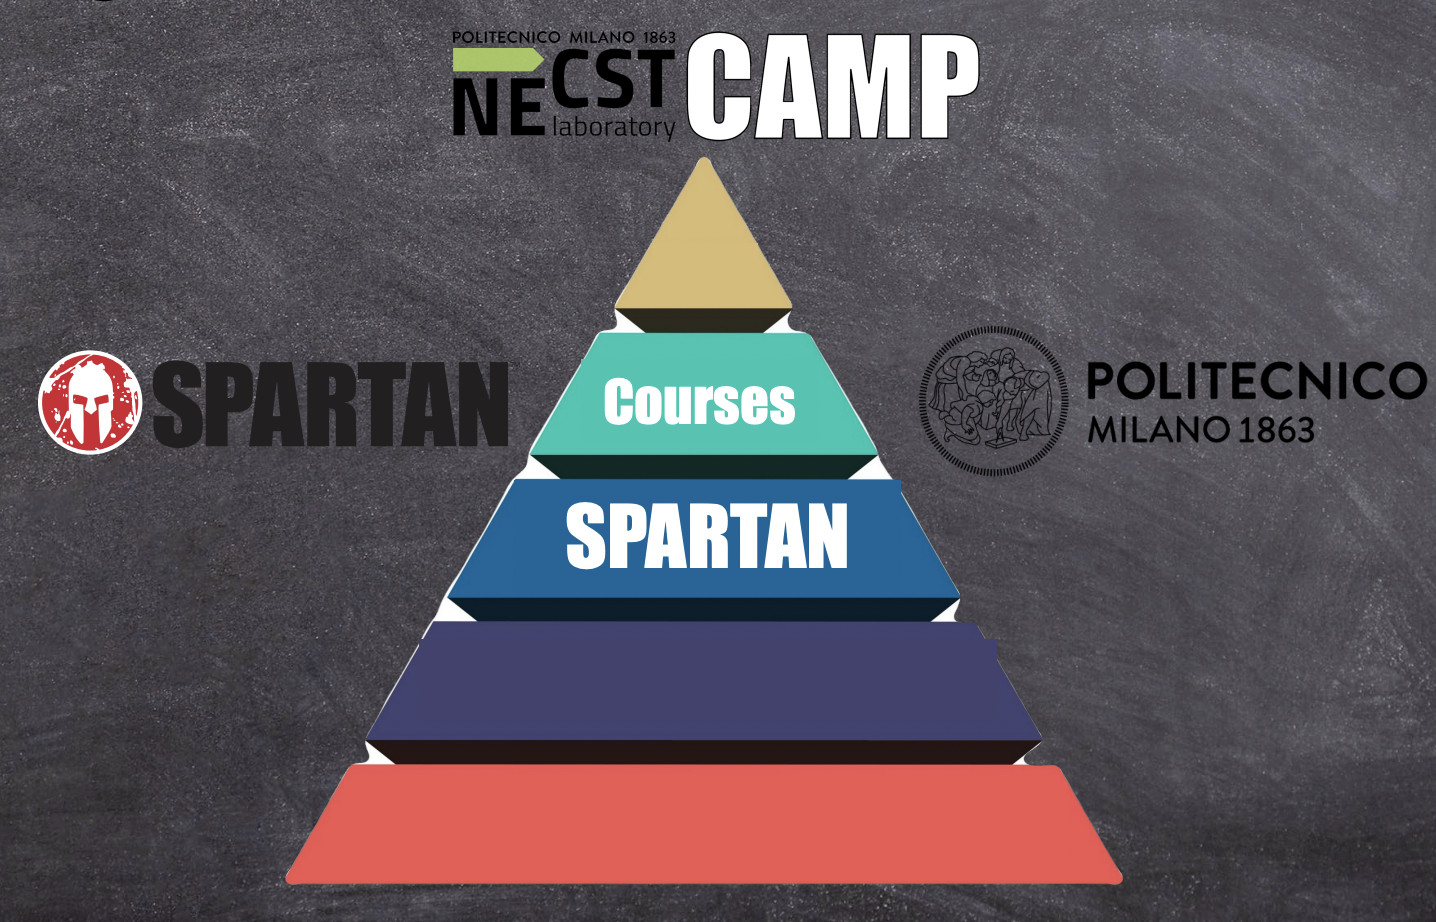
\includegraphics[width=.7\textwidth]{piramide.png}
    \caption{The pyramid of the NecstCAMP}
    \label{fig:my_label}
\end{figure}

\section{Spartan Races} \label{sec:spraces}
Spartan races come in three different categories: Sprint (5km with 20 obstacles), Super (10km with 25 obstacles), and Beast (21km with 30 obstacles). Skipping an obstacle results in penalties such as burpees or penalty loops. Additionally, there are other race variations, including timed races, stadium races, and city races. Interestingly, the number of obstacles does not proportionally increase with the distance covered. These obstacles range from carrying heavy objects and crawling under barbed wire to climbing ropes and scaling walls.

\section{Categories and Teamwork} \label{sec:cat}
Spartan races have three categories: elite, age, and open. Elite participants are professionals, while the age category includes professionals divided by age groups. NecstCAMP students participate in the open category, which is non-competitive unlike the others. During the race, the challenge with oneself combines with teamwork. Playing this challenge with oneself involves making everything measurable, observable, and repeatable. Each race sets a new goal, considering the different conditions presented in various races.

\section{The Spartan Experience} \label{sec:spexp}
Spartan races excel at engaging participants through various means. At the end of each race, participants are rewarded with a t-shirt and a medal (red for Sprint, blue for Super, and green for Beast). Moreover, completing all three race categories within a year earns a Trifecta, symbolized by a one-third circular wedge that, when combined, forms a complete medal. Achieving the Trifecta within a calendar year grants eligibility for the Trifecta Weekend in Sparta. Multiple Trifectas lead to progressively larger medals, representing the number of Trifectas completed. Sparta hosts the Trifecta Weekend in November, which serves as the World Championship. To participate in the Beast category during this event, one must also complete the Super and Sprint races. It is a moment of celebration, honoring athletes who have closed the highest number of Trifectas in their history, such as 30 or 50. Furthermore, if a participant completes 13 Trifectas in a year, they are awarded a shield during the Shield ceremony at Sparta. Each year, the medals feature different symbols, such as a scorpion or jaguar, representing the Spartan theme.

\section{NecstCAMP and Spartan Race Partnership} \label{sec:partn}
NecstCAMP collaborates with Spartan Race Italy, offering students the opportunity to participate in various events throughout the year. Not all events are Trifecta weekends, and there is also a non-competitive category for kids. This partnership allows NecstCAMP students to be involved both as volunteers and as runners. They can alternate between participating in races and volunteering on different weekends. This special relationship between NecstCAMP and Spartan Race stands out, as normally, volunteers usually focus solely on their volunteering duties for a weekend. 
Every volunteer, including NecstCAMP students, receives vouchers for future races after each weekend. However, NecstCAMP students are not allowed to reuse those vouchers, fostering a mutual trust between NecstCAMP and the Spartan Race community.

\section{Training and Progression} \label{sec:prog}
As students engage in successive Spartan races, they are gradually qualified for more challenging courses through a deliberate educational process. They start by running the Sprint race on the first weekend, then have the opportunity to run both the Sprint and Super races on the following weekend. Finally, they become qualified for the Beast race. The idea is that if it is the first year participating in Spartan races, the Trifecta cannot be completed within that year, creating a desire to achieve the milestone without rushing. The game becomes a challenge with oneself.

\section{Preparing for Challenges} \label{sec:prep}
To arrive prepared for a challenge, one must train through crossfit courses, saturday training with Coach Andal, and SGX courses at the Politecnico. Returning to the parallelism between Spartan races and courses, we can identify a key similarity: the phases of practice and performance. Through practice, we apply what we learn and adjust our practice based on what happens during performance. This iterative process of deliberate practice enhances our capabilities. The more we practice, the more skilled we become. 
This principle applies not only to sports but also to academic exams. Deliberate practice involves stepping out of our comfort zone and challenging ourselves with tasks slightly beyond our current abilities, allowing us to gradually expand our potential. In contrast, during performance, we push ourselves beyond our comfort zone to tap into our full potential. However, it is crucial to properly challenge ourselves; the game only works when the challenge matches our abilities, neither too easy nor too difficult.

\section{The Importance of Performance} \label{sec:imp}
During a performance, both the body and mind progress as they precisely execute the required tasks. In contrast, during practice, we maintain full awareness and consciousness. 
The practice in Spartan races corresponds to CrossFit workouts, while in the academic context, it aligns with courses and exercise hours. The performance phase for Spartan races corresponds to the actual races, while in the academic realm, it aligns with exams. Consider what would happen if one attempted to lift a 50kg ball for the first time during a Spartan race or take an exam after a sleepless night. It is natural to feel nervous about performance situations such as exams or projects.

\section{Embracing the Unpredictable} \label{sec:uncont}
We are afraid of performance, but it's interesting that we don't start from performance itself. We fear something that comes afterward, despite the fact that we had full control. This brings up the theme of accepting what you cannot control and working with what depends on you, which is deliberate practice. It's challenging, but there is willingness, a fundamental factor in surpassing our limits.
During practice, there is also event planning for Spartan, which corresponds to scheduling the exam session. So, there are a series of actions that we take to train ourselves even for situations that we cannot predict. During the performance, the unknown remains constant in both contexts: there could be bad weather during a race, just as we may not know what exercises we will encounter in the exam. One significant aspect of performance is the act of applying what we have learned. Performance provides an opportunity to expand our potential by facing appropriate challenges. But what constitutes an appropriate challenge? It is something that allows us to set clear objectives, as demonstrated at NecstCAMP when defining personal goals. To arrive prepared for a challenge, one must train properly and select the right challenge based on their current abilities, setting the right expectations. 
\begin{figure}[h]
    \centering
    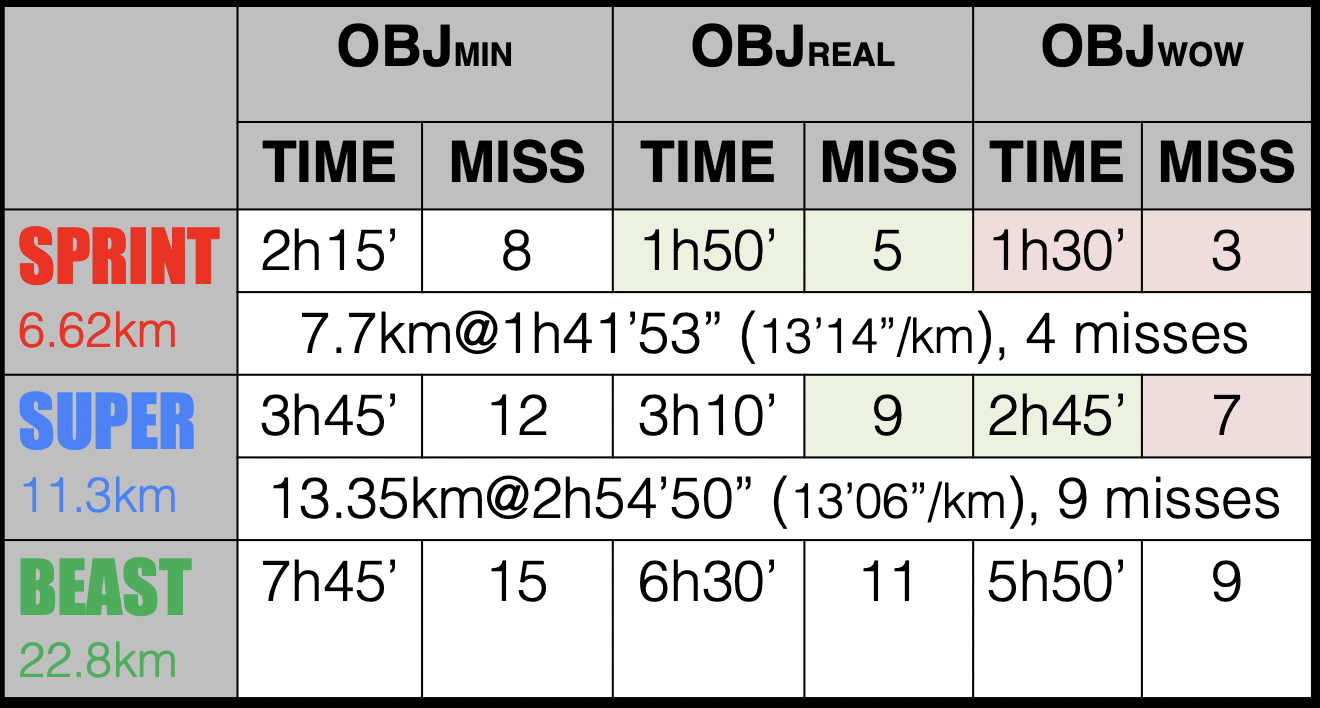
\includegraphics[width=.7\textwidth]{tabella.png}
    \caption{Example of objectives}
    \label{fig:my_label}
\end{figure}
The right expectation translates into defining objectives. This parallels the world of Spartan races, where running a race and training are analogous to taking exams and preparing for them. Defining goals is crucial to create the right challenge, both in Spartan races (measured by time and saved obstacles) and in exams (measured by credits and grades). It is equally important to develop a plan to tackle the challenge strategically, ensuring we do not exhaust all our resources immediately. During the performance, there are sensations that can compromise future performances; for instance, running the first race but having two more races the next day will lead to fatigue. Similarly, refusing to take an exam now, but having another on the same day, will result in additional difficulties. Making impulsive decisions during the performance is not ideal; therefore, creating and adhering to a well-thought-out plan is of utmost importance.
So, what we can control becomes the plan to tackle our challenge and the willingness to follow it. However, it's not possible to control everything. During a Spartan race, we cannot control the extra kilometers we may encounter or the weather alert the night before the race, leading to heavy rain on the following day. Consequently, you find yourself competing on a muddy course that slows you down. You may have practiced crawling under barbed wire in the mud, but you might encounter it uphill or in a river. It cannot be controlled, but with practice, you can be prepared to face it.
\begin{figure}[h]
    \centering
    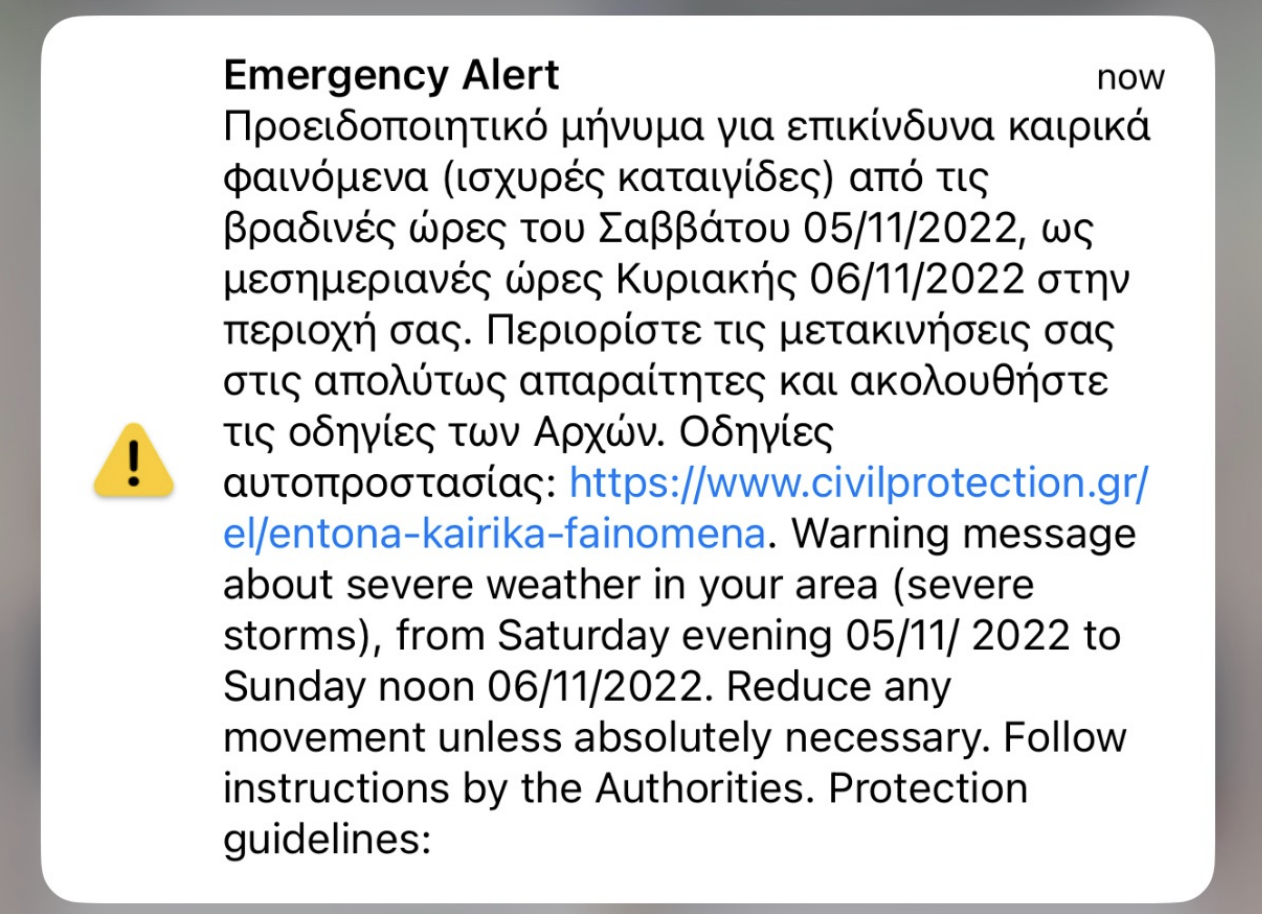
\includegraphics[width=.7\textwidth]{alert.png}
    \caption{Example of an unexpected event}
    \label{fig:my_label}
\end{figure}


\section{Conclusion} \label{sec:concl}
What depends on us? We choose to keep running, to maintain our willpower. To increase our potential, we need to expose ourselves to unfamiliar things, and by choosing to keep running, we can learn something new.


\newpage
\title{\textbf{Bibliography}} \\
\begin{itemize}
\item NecstCAMP meeting of 23/11/2022 held by professor Marco D. Santambrogio
\item NecstCAMP meeting of 26/03/2023 held by professor Marco D. Santambrogio
\end{itemize}


\end{document}


